\documentclass{standalone}
\usepackage{tikz}
\usetikzlibrary{patterns}
\usetikzlibrary{positioning}
\usetikzlibrary{patterns, positioning}
\usetikzlibrary{shapes.misc}
\usepackage[outline]{contour}
\contourlength{1.5pt} 


\begin{document}
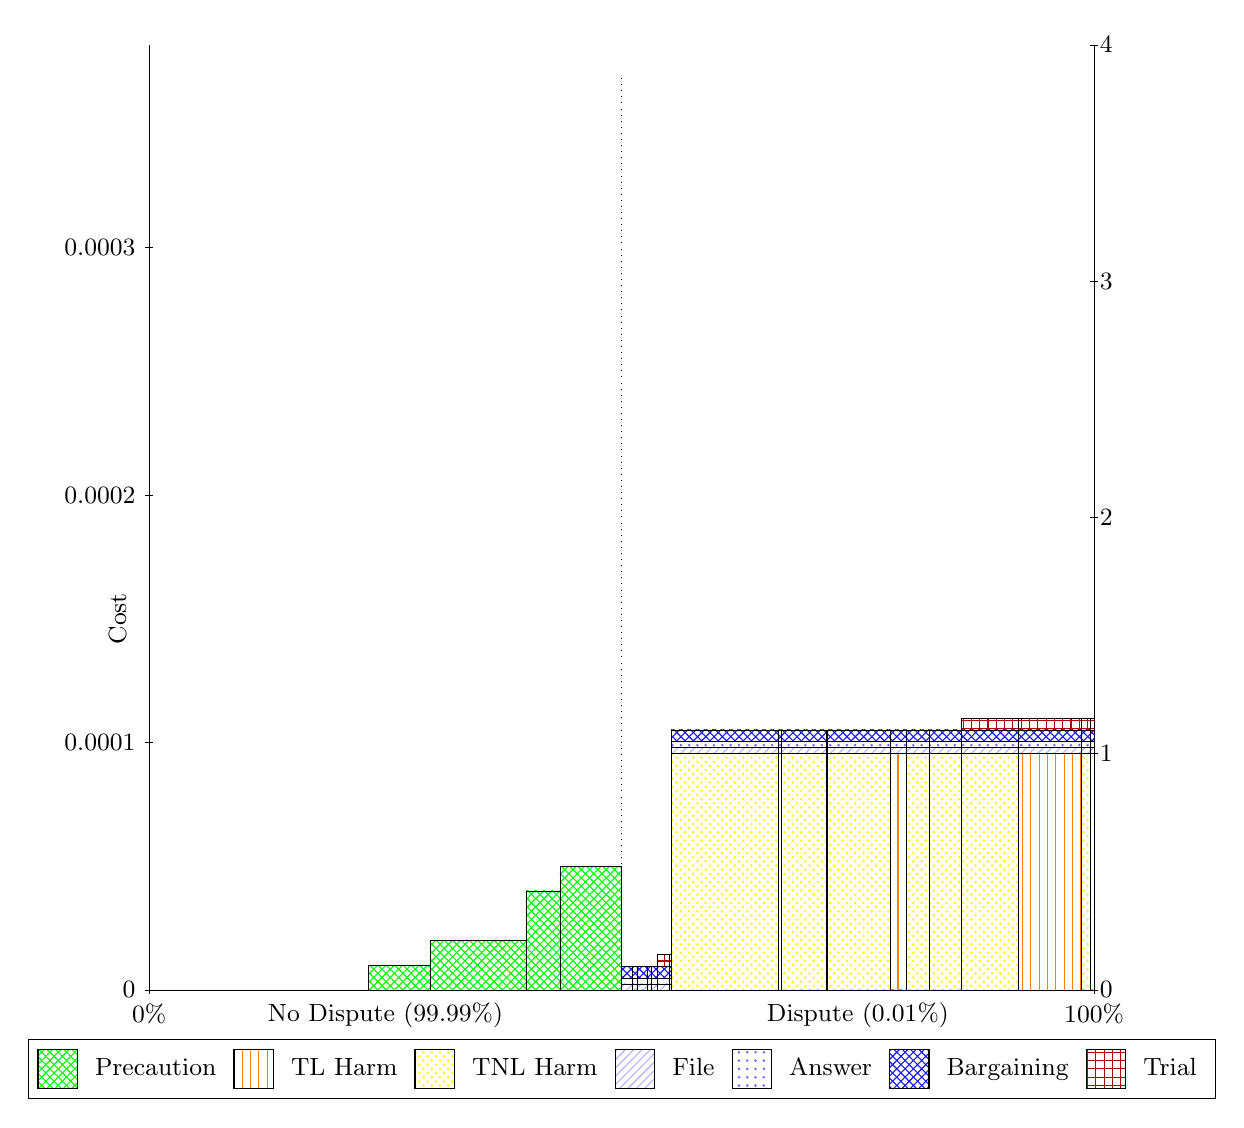
\begin{tikzpicture}
\draw[pattern=crosshatch, pattern color=green,draw=black,very thin] (4.2843,2.5) rectangle (5.0703,2.8141);
\draw[pattern=crosshatch, pattern color=green,draw=black,very thin] (5.0703,2.5) rectangle (6.2843,3.1283);
\draw[pattern=crosshatch, pattern color=green,draw=black,very thin] (6.2843,2.5) rectangle (6.7156,3.7566);
\draw[pattern=crosshatch, pattern color=green,draw=black,very thin] (6.7156,2.5) rectangle (7.5,4.0707);
\draw[pattern=north east lines, pattern color=blue!30,draw=black,very thin] (7.5,2.5) rectangle (7.6394,2.575);
\draw[pattern=dots,  pattern color=blue!60,draw=black,very thin] (7.5,2.575) rectangle (7.6394,2.65);
\draw[pattern=crosshatch,      pattern color=blue!90,draw=black,very thin] (7.5,2.65) rectangle (7.6394,2.8);
\draw[pattern=crosshatch, pattern color=green,draw=black,very thin] (7.6394,2.5) rectangle (7.7034,2.5);
\draw[pattern=north east lines, pattern color=blue!30,draw=black,very thin] (7.6394,2.5) rectangle (7.7034,2.575);
\draw[pattern=dots,  pattern color=blue!60,draw=black,very thin] (7.6394,2.575) rectangle (7.7034,2.65);
\draw[pattern=crosshatch,      pattern color=blue!90,draw=black,very thin] (7.6394,2.65) rectangle (7.7034,2.8);
\draw[pattern=crosshatch, pattern color=green,draw=black,very thin] (7.7034,2.5) rectangle (7.8305,2.5001);
\draw[pattern=north east lines, pattern color=blue!30,draw=black,very thin] (7.7034,2.5001) rectangle (7.8305,2.5751);
\draw[pattern=dots,  pattern color=blue!60,draw=black,very thin] (7.7034,2.5751) rectangle (7.8305,2.6501);
\draw[pattern=crosshatch,      pattern color=blue!90,draw=black,very thin] (7.7034,2.6501) rectangle (7.8305,2.8001);
\draw[pattern=crosshatch, pattern color=green,draw=black,very thin] (7.8305,2.5) rectangle (7.8757,2.5001);
\draw[pattern=north east lines, pattern color=blue!30,draw=black,very thin] (7.8305,2.5001) rectangle (7.8757,2.5751);
\draw[pattern=dots,  pattern color=blue!60,draw=black,very thin] (7.8305,2.5751) rectangle (7.8757,2.6501);
\draw[pattern=crosshatch,      pattern color=blue!90,draw=black,very thin] (7.8305,2.6501) rectangle (7.8757,2.8001);
\draw[pattern=crosshatch, pattern color=green,draw=black,very thin] (7.8757,2.5) rectangle (7.9578,2.5002);
\draw[pattern=north east lines, pattern color=blue!30,draw=black,very thin] (7.8757,2.5002) rectangle (7.9578,2.5752);
\draw[pattern=dots,  pattern color=blue!60,draw=black,very thin] (7.8757,2.5752) rectangle (7.9578,2.6502);
\draw[pattern=crosshatch,      pattern color=blue!90,draw=black,very thin] (7.8757,2.6502) rectangle (7.9578,2.8002);
\draw[pattern=north east lines, pattern color=blue!30,draw=black,very thin] (7.9578,2.5) rectangle (8.11,2.575);
\draw[pattern=dots,  pattern color=blue!60,draw=black,very thin] (7.9578,2.575) rectangle (8.11,2.65);
\draw[pattern=crosshatch,      pattern color=blue!90,draw=black,very thin] (7.9578,2.65) rectangle (8.11,2.8);
\draw[pattern=grid,            pattern color=red!70!black,draw=black,very thin] (7.9578,2.8) rectangle (8.11,2.95);
\draw[pattern=crosshatch, pattern color=green,draw=black,very thin] (8.11,2.5) rectangle (8.1283,2.5);
\draw[pattern=north east lines, pattern color=blue!30,draw=black,very thin] (8.11,2.5) rectangle (8.1283,2.575);
\draw[pattern=dots,  pattern color=blue!60,draw=black,very thin] (8.11,2.575) rectangle (8.1283,2.65);
\draw[pattern=crosshatch,      pattern color=blue!90,draw=black,very thin] (8.11,2.65) rectangle (8.1283,2.8);
\draw[pattern=grid,            pattern color=red!70!black,draw=black,very thin] (8.11,2.8) rectangle (8.1283,2.95);
\draw[pattern=crosshatch dots, pattern color=yellow,draw=black,very thin] (8.1283,2.5) rectangle (9.4936,5.5);
\draw[pattern=north east lines, pattern color=blue!30,draw=black,very thin] (8.1283,5.5) rectangle (9.4936,5.575);
\draw[pattern=dots,  pattern color=blue!60,draw=black,very thin] (8.1283,5.575) rectangle (9.4936,5.65);
\draw[pattern=crosshatch,      pattern color=blue!90,draw=black,very thin] (8.1283,5.65) rectangle (9.4936,5.8);
\draw[pattern=vertical lines, pattern color=orange,draw=black,very thin] (9.4936,2.5) rectangle (9.5221,5.5);
\draw[pattern=north east lines, pattern color=blue!30,draw=black,very thin] (9.4936,5.5) rectangle (9.5221,5.575);
\draw[pattern=dots,  pattern color=blue!60,draw=black,very thin] (9.4936,5.575) rectangle (9.5221,5.65);
\draw[pattern=crosshatch,      pattern color=blue!90,draw=black,very thin] (9.4936,5.65) rectangle (9.5221,5.8);
\draw[pattern=crosshatch, pattern color=green,draw=black,very thin] (9.5221,2.5) rectangle (10.103,2.5);
\draw[pattern=crosshatch dots, pattern color=yellow,draw=black,very thin] (9.5221,2.5) rectangle (10.103,5.5);
\draw[pattern=north east lines, pattern color=blue!30,draw=black,very thin] (9.5221,5.5) rectangle (10.103,5.575);
\draw[pattern=dots,  pattern color=blue!60,draw=black,very thin] (9.5221,5.575) rectangle (10.103,5.65);
\draw[pattern=crosshatch,      pattern color=blue!90,draw=black,very thin] (9.5221,5.65) rectangle (10.103,5.8);
\draw[pattern=crosshatch, pattern color=green,draw=black,very thin] (10.103,2.5) rectangle (10.11,2.5);
\draw[pattern=vertical lines, pattern color=orange,draw=black,very thin] (10.103,2.5) rectangle (10.11,5.5);
\draw[pattern=north east lines, pattern color=blue!30,draw=black,very thin] (10.103,5.5) rectangle (10.11,5.575);
\draw[pattern=dots,  pattern color=blue!60,draw=black,very thin] (10.103,5.575) rectangle (10.11,5.65);
\draw[pattern=crosshatch,      pattern color=blue!90,draw=black,very thin] (10.103,5.65) rectangle (10.11,5.8);
\draw[pattern=crosshatch, pattern color=green,draw=black,very thin] (10.11,2.5) rectangle (10.912,2.5001);
\draw[pattern=crosshatch dots, pattern color=yellow,draw=black,very thin] (10.11,2.5001) rectangle (10.912,5.5001);
\draw[pattern=north east lines, pattern color=blue!30,draw=black,very thin] (10.11,5.5001) rectangle (10.912,5.5751);
\draw[pattern=dots,  pattern color=blue!60,draw=black,very thin] (10.11,5.5751) rectangle (10.912,5.6501);
\draw[pattern=crosshatch,      pattern color=blue!90,draw=black,very thin] (10.11,5.6501) rectangle (10.912,5.8001);
\draw[pattern=crosshatch, pattern color=green,draw=black,very thin] (10.912,2.5) rectangle (11.114,2.5001);
\draw[pattern=vertical lines, pattern color=orange,draw=black,very thin] (10.912,2.5001) rectangle (11.114,5.5001);
\draw[pattern=north east lines, pattern color=blue!30,draw=black,very thin] (10.912,5.5001) rectangle (11.114,5.5751);
\draw[pattern=dots,  pattern color=blue!60,draw=black,very thin] (10.912,5.5751) rectangle (11.114,5.6501);
\draw[pattern=crosshatch,      pattern color=blue!90,draw=black,very thin] (10.912,5.6501) rectangle (11.114,5.8001);
\draw[pattern=crosshatch, pattern color=green,draw=black,very thin] (11.114,2.5) rectangle (11.408,2.5001);
\draw[pattern=crosshatch dots, pattern color=yellow,draw=black,very thin] (11.114,2.5001) rectangle (11.408,5.5001);
\draw[pattern=north east lines, pattern color=blue!30,draw=black,very thin] (11.114,5.5001) rectangle (11.408,5.5751);
\draw[pattern=dots,  pattern color=blue!60,draw=black,very thin] (11.114,5.5751) rectangle (11.408,5.6501);
\draw[pattern=crosshatch,      pattern color=blue!90,draw=black,very thin] (11.114,5.6501) rectangle (11.408,5.8001);
\draw[pattern=crosshatch, pattern color=green,draw=black,very thin] (11.408,2.5) rectangle (11.816,2.5002);
\draw[pattern=crosshatch dots, pattern color=yellow,draw=black,very thin] (11.408,2.5002) rectangle (11.816,5.5002);
\draw[pattern=north east lines, pattern color=blue!30,draw=black,very thin] (11.408,5.5002) rectangle (11.816,5.5752);
\draw[pattern=dots,  pattern color=blue!60,draw=black,very thin] (11.408,5.5752) rectangle (11.816,5.6502);
\draw[pattern=crosshatch,      pattern color=blue!90,draw=black,very thin] (11.408,5.6502) rectangle (11.816,5.8002);
\draw[pattern=crosshatch dots, pattern color=yellow,draw=black,very thin] (11.816,2.5) rectangle (12.541,5.5);
\draw[pattern=north east lines, pattern color=blue!30,draw=black,very thin] (11.816,5.5) rectangle (12.541,5.575);
\draw[pattern=dots,  pattern color=blue!60,draw=black,very thin] (11.816,5.575) rectangle (12.541,5.65);
\draw[pattern=crosshatch,      pattern color=blue!90,draw=black,very thin] (11.816,5.65) rectangle (12.541,5.8);
\draw[pattern=grid,            pattern color=red!70!black,draw=black,very thin] (11.816,5.8) rectangle (12.541,5.95);
\draw[pattern=vertical lines, pattern color=orange,draw=black,very thin] (12.541,2.5) rectangle (13.338,5.5);
\draw[pattern=north east lines, pattern color=blue!30,draw=black,very thin] (12.541,5.5) rectangle (13.338,5.575);
\draw[pattern=dots,  pattern color=blue!60,draw=black,very thin] (12.541,5.575) rectangle (13.338,5.65);
\draw[pattern=crosshatch,      pattern color=blue!90,draw=black,very thin] (12.541,5.65) rectangle (13.338,5.8);
\draw[pattern=grid,            pattern color=red!70!black,draw=black,very thin] (12.541,5.8) rectangle (13.338,5.95);
\draw[pattern=crosshatch, pattern color=green,draw=black,very thin] (13.338,2.5) rectangle (13.453,2.5);
\draw[pattern=crosshatch dots, pattern color=yellow,draw=black,very thin] (13.338,2.5) rectangle (13.453,5.5);
\draw[pattern=north east lines, pattern color=blue!30,draw=black,very thin] (13.338,5.5) rectangle (13.453,5.575);
\draw[pattern=dots,  pattern color=blue!60,draw=black,very thin] (13.338,5.575) rectangle (13.453,5.65);
\draw[pattern=crosshatch,      pattern color=blue!90,draw=black,very thin] (13.338,5.65) rectangle (13.453,5.8);
\draw[pattern=grid,            pattern color=red!70!black,draw=black,very thin] (13.338,5.8) rectangle (13.453,5.95);
\draw[pattern=crosshatch, pattern color=green,draw=black,very thin] (13.453,2.5) rectangle (13.5,2.5);
\draw[pattern=vertical lines, pattern color=orange,draw=black,very thin] (13.453,2.5) rectangle (13.5,5.5);
\draw[pattern=north east lines, pattern color=blue!30,draw=black,very thin] (13.453,5.5) rectangle (13.5,5.575);
\draw[pattern=dots,  pattern color=blue!60,draw=black,very thin] (13.453,5.575) rectangle (13.5,5.65);
\draw[pattern=crosshatch,      pattern color=blue!90,draw=black,very thin] (13.453,5.65) rectangle (13.5,5.8);
\draw[pattern=grid,            pattern color=red!70!black,draw=black,very thin] (13.453,5.8) rectangle (13.5,5.95);
\draw[black,very thin] (1.5,2.5) -- (1.5,14.5);
\node[font=\small,rotate=90,text=black, anchor=center] at (1.1, 7.2121) {Cost};
\draw[black,very thin] (1.45,2.5) -- (1.55,2.5);
\node[font=\small,text=black, anchor=east] at (1.45, 2.5) {0};
\draw[black,very thin] (1.45,5.6414) -- (1.55,5.6414);
\node[font=\small,text=black, anchor=east] at (1.45, 5.6414) {0.0001};
\draw[black,very thin] (1.45,8.7828) -- (1.55,8.7828);
\node[font=\small,text=black, anchor=east] at (1.45, 8.7828) {0.0002};
\draw[black,very thin] (1.45,11.924) -- (1.55,11.924);
\node[font=\small,text=black, anchor=east] at (1.45, 11.924) {0.0003};

\draw[black,dotted,very thin] (7.5,2.86) -- (7.5,14.14);
\draw[black,very thin] (13.5,2.5) -- (13.5,14.5);
\draw[black,very thin] (13.45,2.5) -- (13.55,2.5);
\node[font=\small,text=black, anchor=west] at (13.45, 2.5) {0};
\draw[black,very thin] (13.45,5.5) -- (13.55,5.5);
\node[font=\small,text=black, anchor=west] at (13.45, 5.5) {1};
\draw[black,very thin] (13.45,8.5) -- (13.55,8.5);
\node[font=\small,text=black, anchor=west] at (13.45, 8.5) {2};
\draw[black,very thin] (13.45,11.5) -- (13.55,11.5);
\node[font=\small,text=black, anchor=west] at (13.45, 11.5) {3};
\draw[black,very thin] (13.45,14.5) -- (13.55,14.5);
\node[font=\small,text=black, anchor=west] at (13.45, 14.5) {4};

\draw[black,very thin] (1.5,2.5) -- (13.5,2.5);
\draw[black,very thin] (1.5,2.45) -- (1.5,2.55);
\node[font=\small,text=black, anchor=north] at (1.5, 2.45) {0\%};
\draw[black,very thin] (13.5,2.45) -- (13.5,2.55);
\node[font=\small,text=black, anchor=north] at (13.5, 2.45) {100\%};

\node[font=\small,text=black,anchor=south] at (4.5, 1.9) {No\ Dispute\ (99.99\%)};
\node[font=\small,text=black,anchor=south] at (10.5, 1.9) {Dispute\ (0.01\%)};
\draw (7.5,2.5) node (B) {};
\begin{scope}[align=center]
\matrix[scale=0.5,draw=black,below=0.5cm of B,nodes={draw},column sep=0.1cm]{
\node[rectangle,draw,minimum width=0.5cm,minimum height=0.5cm,pattern=crosshatch, pattern color=green]{}; & \node[draw=none,font=\small,text=black]{Precaution}; &
\node[rectangle,draw,minimum width=0.5cm,minimum height=0.5cm,pattern=vertical lines, pattern color=orange]{}; & \node[draw=none,font=\small,text=black]{TL Harm}; &
\node[rectangle,draw,minimum width=0.5cm,minimum height=0.5cm,pattern=crosshatch dots, pattern color=yellow]{}; & \node[draw=none,font=\small,text=black]{TNL Harm}; &
\node[rectangle,draw,minimum width=0.5cm,minimum height=0.5cm,pattern=north east lines, pattern color=blue!30]{}; & \node[draw=none,font=\small,text=black]{File}; &
\node[rectangle,draw,minimum width=0.5cm,minimum height=0.5cm,pattern=dots,  pattern color=blue!60]{}; & \node[draw=none,font=\small,text=black]{Answer}; &
\node[rectangle,draw,minimum width=0.5cm,minimum height=0.5cm,pattern=crosshatch,      pattern color=blue!90]{}; & \node[draw=none,font=\small,text=black]{Bargaining}; &
\node[rectangle,draw,minimum width=0.5cm,minimum height=0.5cm,pattern=grid,            pattern color=red!70!black]{}; & \node[draw=none,font=\small,text=black]{Trial}; \\\\
};\end{scope}

\end{tikzpicture}
\end{document}